This chapter concerns the most important parts about how this project has been implemented. It has been split into several sections.

\Mathias{Write shortly about the implementation Chapter}
\Mathias{Less calculations on the drone, better to move to another computer/cluster with more power than the drone has available from its battery}
\Mathias{Image of camera and drone seen from the side. Show what happens to the drones position estimation when it drifts down/up}

\section{CAN implementation}
\subsection{Introduction}
In order to spoof the onboard GPS, the CAN-bus was chosen as input to AQ. 
The CAN-bus is already implemented and widely used on a ViaCopter drone to communicate between AQ and hardware like ESCs, PDB etc. Much time was spend reading through the source code and trying to figure out how the protocol works.
The developers behind AQ says, that the code is the documentation and thereby have not written any real documentation. \\
Figuring out how it works was done using debugging utilities such as breakpoints and looking at the content of the different memory locations in CrossWorks.
To further investigate the protocol a PEAK-CAN adapter were connected to a Ladybird drone and several python scripts were developed to send and receive messages from AQ. \\
The author did not go into details about messages used between AQ $\leftrightarrow$ ESC's and AQ $\leftrightarrow$ OSD.\\


\subsection{CAN Protocol description}
A Peak-CAN adapter were used throughout the project. It supports High-speed ISO 11898-2\footnote{\url{http://www.peak-system.com/PCAN-USB.199.0.html?&L=1}} which is a standard that states the properties of physical layer. 
Its max speed is 1 mbit which is the speed AQ uses to communicate on the CAN-bus. 
AQ uses CAN 2.0B which has 29 identifier bits.
AQ is not using an existing protocol on top of ISO 11898-2. The developers created their own to suit their needs.\\

\subsubsection{Identifier bits}
A Generic look at a AQ CAN messages can be seen in table \ref{tab:can_identifier_bits}.
The normal function of the identifier bits is the priority of the messages.
A CAN controller can then be setup to only allow certain messages to be processed depending on their identifier bits.
The identification bits has been split up in AQ to contain information about the sender, receiver etc. Which is not normally saved information in a CAN message.
\begin{table}[H]
\resizebox{\textwidth}{!}{%
	\begin{tabular}{|c|c|c|c|c|c|c|c|}
	\hline
	\multicolumn{8}{|c|}{CAN Message} \\ 
	\hline
	 \multicolumn{7}{|c|}{Identfier bits [29 bits]} &  		\multicolumn{1}{c|}{Data bits [max 64 bits]} \\
	 \hline
	 LCC [28:27] & TT [26] & FID [25:22] & DOC [21:16] & SOID 	[15:11] & TID [10:16] & SEID [5:0] & \\
	\hline
\end{tabular}}
	\caption{Table shows the identifier bits used in AutoQuad CAN messages}
	\label{tab:can_identifier_bits}
\end{table}

In figure \ref{tab:abbri_can_msg} the abbreviations can be seen.
\begin{table}[H]
		\begin{tabular}{|l|l|}
		\hline
		LCC & Logical Communications Channe \\
\hline
		TT & Target Type \\
\hline
		FID & Function ID \\
\hline
		DOC & Data Object Code \\
\hline
		SOID & Source ID \\
\hline
		TID & Target ID \\
\hline
		SEID & Sequence ID \\
\hline
		\end{tabular}
		\caption{Table shows 
abbreviations used in table \ref{tab:can_identifier_bits}}
		\label{tab:abbri_can_msg}
\end{table}

Each of the elements in an AQ messages will be explained how they are used in AQ. \\

\subsubsection{Logic Communication Channel}
LCC is the priority of the message. 
To understand how LCC works, one needs to look into CAN arbitration.
As stated in ISO-11898-2, a 0 is the dominant bit and a 1 is the recessive bit.
The example in figure \ref{tab:can_arbitration} shows two nodes each transmitting a packet.
The arbitration only happens during the transmission of the identifier bits.
In the example on bit 8, Node 16 losses the arbitration and stops transmitting.
Node 15 keeps transmitting its packet because it has lower identifier bits and thereby higher priority.
\begin{figure}[H]
    \center
    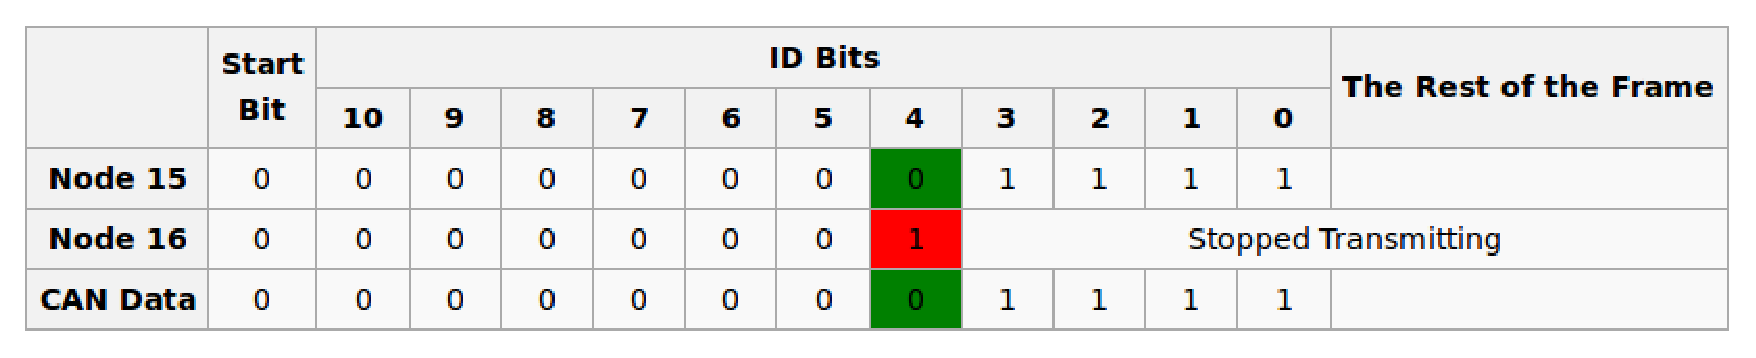
\includegraphics[width=1\textwidth]{graphics/can_arbitration.eps}
    \caption{Example of CAN arbitration where node 15 has the lowest ID and thereby highest priority}
    \label{tab:can_arbitration}
\end{figure}
\newpage
LLC in a message can take one of the defines in code \ref{code:llc_defines}
\begin{lstlisting}[language = c, caption = LLC defines, label=code:llc_defines]
#define CAN_LCC_EXCEPTION   ((uint32_t)0x0<<30)
#define CAN_LCC_HIGH        ((uint32_t)0x1<<30)
#define CAN_LCC_NORMAL      ((uint32_t)0x2<<30)
#define CAN_LCC_INFO        ((uint32_t)0x3<<30)
\end{lstlisting}

\begin{table}[H]
\centering
\caption{Table showing the 4 types of priority in AQ}
\label{my-label}
\begin{tabular}{|l|l|l|}
\hline
\textbf{Name} & \textbf{Value} & \textbf{Priority (lowest first)} \\ \hline
EXCEPTION     & 0000           & 0                 \\ \hline
HIGH          & 0001           & 1                 \\ \hline
NORMAL        & 0010           & 2                 \\ \hline
INFO          & 0011           & 3                 \\ \hline
\end{tabular}
\end{table}

\subsubsection{Target Type}
Target type can either be “node” or “group” depending on if the receiver(s) is one or more nodes. 
\begin{lstlisting}[language = c, caption = Target type defined in AQ, label=code:target_types]
#define CAN_TT_GROUP        ((uint32_t)0x0<<29)
#define CAN_TT_NODE         ((uint32_t)0x1<<29)
\end{lstlisting}
The GROUP is used when AQ sends its reset-msg upon startup.\\
When the authors node send a sensor-measure to AQ it will be of type NODE.
\subsubsection{Function ID}

Function ID describes the function of the CAN message. If it is a PING, ACK, NACK, etc.
It simply states the function of packet so the receiver node knows what to do with the message.
Different types of functions can be seen in code \ref{code:function_defines}
\begin{lstlisting}[language = c, caption = Excerpts from AQ's list of function defines, label=code:function_defines]
#define CAN_FID_RESET_BUS		((uint32_t)0x0<<25)
#define CAN_FID_ACK				((uint32_t)0x1<<25)
#define CAN_FID_REQ_ADDR		((uint32_t)0x7<<25)
#define CAN_FID_GRANT_ADDR	((uint32_t)0x8<<25)
\end{lstlisting}

Table \ref{tab:fid_descriptions} describes the FIDs shown in code \ref{code:function_defines}.
\begin{table}[H]
\centering
\caption{Descriptions of the FIDs mentioned in code \ref{code:function_defines}}
\label{tab:fid_descriptions}
\resizebox{\textwidth}{!}{%
\begin{tabular}{@{}|l|l|@{}}
\toprule
\textbf{FID}          & \textbf{Description}                                                               \\ \midrule
CAN\_FID\_RESET\_BUS  & Message sent by AQ when powered up                                                 \\ \midrule
CAN\_FID\_ACK         & Message sent to AQ when acknowledging a received message                           \\ \midrule
CAN\_FID\_REQ\_ADDR   & Messaged used when a node on the bus tries to register itself as a node on the bus \\ \midrule
CAN\_FID\_GRANT\_ADDR & Messaged sent by AQ when it registers a node as a node on the bus.                 \\ \bottomrule
\end{tabular}
}
\end{table}

Table \ref{tab:fid_descriptions} shows a description of the 4 FIDs used when a node is registered. 

\subsubsection{Data Object Code}
Comming.. Kind of parameter to FID
\Mathias{eksempel på hvordan de bliver brugt i koden - vise function id i switch/case}
\Mathias{Dscripe how the node is created on the BUS}

\subsubsection{Source/Target/Network ID}
When referred to source/target ID but without respect to either sender or receiver but just a CAN-node, then it is referred to as NetworkId. When a node registers itself in AQ, it gets assigned a NetworkId.

\subsubsection{Sequence ID}
The sequence id is incremented on transmission of each message. It is used when eg. 
A CAN-node sends a reply to a get-message, it is then including the sequence id of the get-message so AQ knows what it receives a reply for.

\subsubsection{Data bits}
The data bytes does not have a general definition, it depends on the function id. With some FIDs the data field may contain additional parameters.\\ \\
Eg. When FID is CAN\_FID\_REQ\_ADDR, data has the fields shown in table \ref{tab:packet_from_node}
\begin{table}[H]
\centering
\caption{Packet sent from node when registering in AQ}
\label{tab:packet_from_node}
\begin{tabular}{@{}|c|c|c|c|c|c|c|c|@{}}
\toprule
\multicolumn{8}{|c|}{64 bits}                           \\ \midrule
0 & 0 & CanId & CanType & UUID3 & UUID2 & UUID1 & UUID0 \\
\midrule
7 & 6 & 5 & 4 & 3 & 2 & 1 & 0 \\ \bottomrule
\end{tabular}
\end{table}

\textbf{UUID} is a unique address generated by each node on the bus. In ESC32v2\footnote{\url{https://github.com/bn999/esc32/blob/master/onboard/can.c}} the address is calculated using XXH-hashing algorithm. The algorithm generates a 32 bit hash from a given input value and a salt.
The input to XXH in ESC32v2 is the unique ID that every ARM in the STMF32\footnote{\url{http://www2.st.com/content/ccc/resource/technical/document/reference_manual/59/b9/ba/7f/11/af/43/d5/CD00171190.pdf/files/CD00171190.pdf/jcr:content/translations/en.CD00171190.pdf}}
 family has. Code \ref{code:xxh_canesc32v2} shows how it is implemented in AQ.

\begin{lstlisting}[language = c, caption = Snippet showing UUID generated in ESC32v2, label=code:xxh_canesc32v2]
can.h:20
#define CAN_UUID	0x1FFFF7E8

can.c:753
canData.uuid = XXH32((void *)CAN_UUID, 3*4, 0);
\end{lstlisting}

\textbf{CanType} is the type of the node trying to register. Eq. SENSOR, ESC and SERVO.  \\

\textbf{CanID} is the number of the CanType node trying to register. When an ESC32v2 is trying to register it sends CanId as the ESC number ranging from 1 to the number of ESC's mounted on the drone. The CanID is assign to each ESC manually as part of the configuring.

% redefine the \mess so that \_ works...
\renewcommand{\mess}[4][0]{
  \stepcounter{seqlevel}
  \path
  (#2)+(0,-\theseqlevel*\unitfactor-0.7*\unitfactor) node (mess from) {};
  \addtocounter{seqlevel}{#1}
  \path
  (#4)+(0,-\theseqlevel*\unitfactor-0.7*\unitfactor) node (mess to) {};
  \draw[->,>=angle 60] (mess from) -- (mess to) node[midway, above]
  {#3};
}

\subsection{Registering a node in AQ}

.....
\begin{figure}[H]
    \center
      \begin{adjustbox}{max width=0.5\textwidth}
	\begin{sequencediagram}
	  \newthread{0.4}{pynode}{ROS-node}
	  \newthread{7}{autoquad}{AutoQuad}

	  \mess[1]{autoquad}{CAN\_FID\_RESET\_BUS}{pynode}

	  \begin{call}[3]{autoquad}{Wait(100ms)}{autoquad}
			\postlevel
			\postlevel
			\mess{pynode}{CAN\_FID\_REQ\_ADDR}{autoquad}
			\postlevel
			\mess{autoquad}{CAN\_FID\_GRANT\_ADDR}{pynode}
	  \end{call}
	  \mess{autoquad}{CanTelemeryValue}{pynode}
	  \mess{pynode}{ACKValue*}{autoquad}
	  \postlevel

  	  \mess{autoquad}{CanTelemetryRate}{pynode}
  	  \mess{pynode}{ACKRate}{autoquad}
	\end{sequencediagram}
	\end{adjustbox}
	\label{fig:protocol_req_node}
	\caption{Registering a new node in AQ}
\end{figure}

Test of sending sensor data
\begin{figure}[H]
    \center
    \includegraphics[width=0.8\textwidth]{graphics/test_can_spoof_current.png}
    \caption{Test of python CAN test}
    \label{fig:PCB_block}
\end{figure}
  can0  00000000   [0] 
  can0  01C00000   [8]  EF BE AD DE 03 09 00 00
  can0  0E000041   [6]  EF BE AD DE 00 00
  can0  14CD0042   [2]  00 08
  can0  14CC0043   [2]  0A 00



seq tæller op så rate/value bliver acknowledged
  can0  00000000   [0] 
  can0  01C00000   [8]  EF BE AD DE 03 09 00 00
  can0  0E000041   [6]  EF BE AD DE 00 00
  can0  14CD0042   [2]  00 08
  can0  00400002   [8]  00 00 00 00 00 00 00 00
  can0  14CC0043   [2]  0A 00
  can0  00400003   [8]  00 00 00 00 00 00 00 00


\section{Communication flow}
\begin{table}[H]
\centering

\begin{tabularx}{0.75\textwidth}{@{}|X|X|X|X|X|X|@{}}
\toprule
Content & Lat    & Lon    & Height & DOP   & CRC-16  \\ \midrule
Datatype    & double & double & float  & float & uint16\_t \\ \midrule
Bytes    & 31:24  & 23:16   & 15:8    & 7:4 & 3:0 \\ \bottomrule
\end{tabularx}
\Mathias{Ændre 0:3 til 0:1 da en uint16\_t kun tager 2 bytes og ikke 4}
\caption{Message sent from PC to ESP8266}
\label{my-label}
\end{table}

\section{Vision based localization}
\begin{itemize}
	\item Introduction to section(chapter)
	\item Why use vision as lozalization. cheap, no expensive sensors.
	\item About the MarkerLocator(out of scope), how it works,(Overview - not in depth, why it's slow, how window-mode works) how it's implemented, scalability.
	\item Quality meassure, why is it nessecary.
	\item How I arrived to a good way of meassureing the found marker.
	\item One drone detection
	\item Two drones detection, different ways of detecting orders.
	\item Implementation in ROS, splitting into different nodes.	optimization
\end{itemize}

\begin{figure}[H]
    \center
    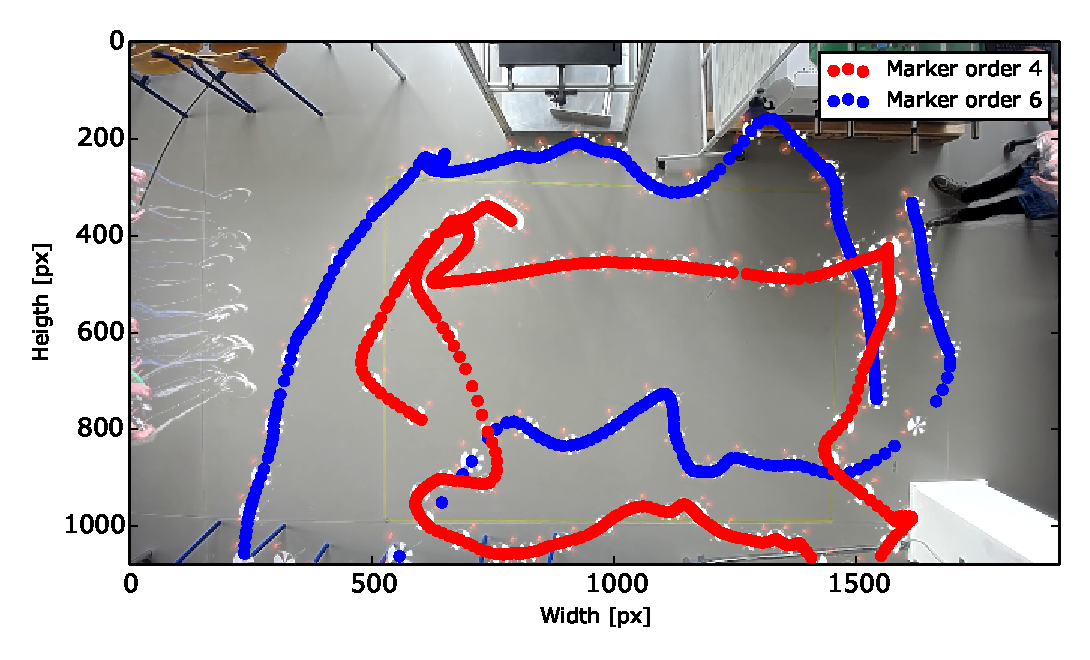
\includegraphics[width=1\textwidth]{graphics/test.eps}
  \label{fig:boat1}
  \caption{Figure showing every 7'th frame merged into one frame combined with the tracked positions of the drones}
\end{figure}
\Mathias{Smaller dot size - almost impossible to see the drone in the frames..}

\Mathias{Red is above blue, not because the drone wasn't detcted}
\Mathias{WIfi test distance, see what happens to latency}
\newpage

\section{Software}
\textit{This capter concerns only the Atmega.  The ESP module will be descriped in section \ref{sec:esp_firmware}} \\
In order to have a timing on the At90CAN128 a scheduler was chosen and implemented.
The list below shows 3 different types of scheduler that was considered.
\begin{itemize}
	\item Real-time Operating System(RTOS) provides strict timing but at the cost of overhead. A RTOS runs task in a "parallel" environment. Each task runs in a loop and the RTOS scheduler will do context switching when needed. Using a RTOS requires mutexes and semaphores to protect shared resources which increases the complexity and amount of overhead
	\item Super-Loop provides no timing at all, but process data as fast as possible. It does not do any context switching and does not require mutexes or semaphores and  and thereby takes no overhead.
	\item Run-To-Complete(RTCS) scheduler is a mix of the two other schedulers. It works by waiting for a tick generated by a hardware timer and then starts executing all tasks from the beginning. The order of the task matters if there is dependency between the tasks but also to make sure the task requiring the most precise timing is at the beginning of the list of the tasks. All tasks have to be finished executing before the next tick is giving in order to avoid timing is ruined.
\end{itemize}
The RTCS was chosen since it provides timing without the overhead created when doing context-switching and the need of mutex and semaphores. It further reduces the code-complexity.\\

\Mathias{A little description about the scheduler implementation. Add tasks, and run the scheduler. Show how it waits for tick and the runs through all of the tasks that is in RUN state.}

It was decided to implement the code in tasks to make a low coupling between the functionalities. This makes it easier to maintain and expand later of if needed. The task diagram shown in figure \ref{fig:task_diagram_atmega} shows the tasks and how they do intertask communication.


\begin{figure}[H]
    \center
    \includegraphics[width=0.9\textwidth]{graphics/task_diagram.png}
  \caption{Tasks diagram showing overview of the running tasks on the At90Can128}
    \label{fig:task_diagram_atmega}
\end{figure}
A small description of each of the tasks is given below:
\begin{itemize}
\item \textbf{ is\_alive\_task} Toggles the green led to make sure the scheduler is running. In case of stack overflow, memoryleak or any other error, the Atmega will freeze and it will easily be detectable since the green led stops blinking
\item \textbf{ uart0\_tx\_task} Responsible of sending characters in the uart0\_tx queue.
\item \textbf{ uart0\_rx\_task} Responsible of checking if any characters in the uart-receive buffer is available. If any, put them into the uart0\_rx queue
\item \textbf{ uart1\_tx\_task} Responsibile as uart\_0\_tx\_task
\item \textbf{ uart1\_rx\_task} Responsibile as uart\_0\_rx\_task
\item \textbf{ can\_rx\_task} Responsible of checking if a CAN-message is available in the MOB. If any put them into the CAN\_rx\_queue
\item \textbf{ can\_tx\_task} Responsible of transmitting messages available in the CAN\_tx\_queue
\item \textbf{ aq\_node\_task} Responsible of registering the node when AQ boots.
\item \textbf{ task\_slip\_decode\_crc\_task} Responsible of removing SLIP characters and run CRC
\item \textbf{ aq\_spoof\_task} Responsible of converting and transmitting received GPS messages from uart1.
\end{itemize}
\Mathias{Add description of slip and crc task, maybe also spoof and node, not sure..}

\subsubsection*{Test of RTCS timing}
In order to test the timing of the scheduler, a led\_task was written. The task can be seen in code \ref{code:test_scheduler}
\begin{lstlisting}[language = c, caption = RTCS task used in timing test, label=code:test_scheduler]
void is_alive_task(uint8_t my_state){

	// Write to UART0
	UDR0 = my_state+'0';

	switch(my_state){
	case 0:
		INT_LED_ON_GREEN;
		INT_LED_OFF_RED;
		INT_LED_OFF_BLUE;
	    set_state( 1 );
		break;
	case 1:
		INT_LED_OFF_GREEN;
		INT_LED_ON_RED;
		INT_LED_OFF_BLUE;
	    set_state( 2 );
		break;
	case 2:
		INT_LED_OFF_GREEN;
		INT_LED_OFF_RED;
		INT_LED_ON_BLUE;

		// Set next state
	    set_state( 0 );
		break;
	}
	// Wait one second
	wait( 1000 );
}
\end{lstlisting}

The test was done by writing the current state of the task to UART0.\\ A python script were made that measures the time between each character received. The script can be seen in code \ref{code:test_rtcs_python}.
\begin{lstlisting}[language = python, caption = Python code used to measure time between received byte, label=code:test_rtcs_python]
#!/usr/bin/python
import serial
import time

ser = serial.Serial( port='/dev/ttyUSB0', baudrate=57600 )

t = time.time()
while True:
    char =  ser.read(1):
    print time.time() - t, ","
    t = time.time()

ser.close()
\end{lstlisting}
The output of the script were redirected to a file. After receiving 700 bytes the standard deviation and mean was calculated using matlab.
The mean is 1.0089 sec with a standard deviation of 0.0042 sec.

Part of the variance is caused by the inaccuracy of the timing on the PC running the python code. If a more accurate measure was needed, a scope could be attached to the $\mu$C's GPIO. Each time the scheduler enters the task the GPIO should be set high, and when it exists the GPIO should be set low. The scopes at SDU is capable of telling the variance of the off signal. \\
It can be concluded that the scheduler performs well.
\section{Hardware}
\subsection{Introduction}
This secion will go in depth about the extentionboard created as ab addon to the AQ M4 board. The extentionboard was developed to act as a bridge between PC and the CAN-bus using wireless communication in order to send GPS coordinates from the PC to the Drones.\\

The block schematic shown in figure \ref{fig:PCB_block} was created by the auther of the report. It was then given to Carsten Albertsen who created the schematic and did rest of the creation of the PCB.
\\
\Mathias{Create schematic appendix}
\Mathias{Add GPS, WIFI, PCB, PC to forkortelses liste}
\Mathias{Thanks to Carsten Albertsen for PCB development}
\begin{figure}[H]
    \center
    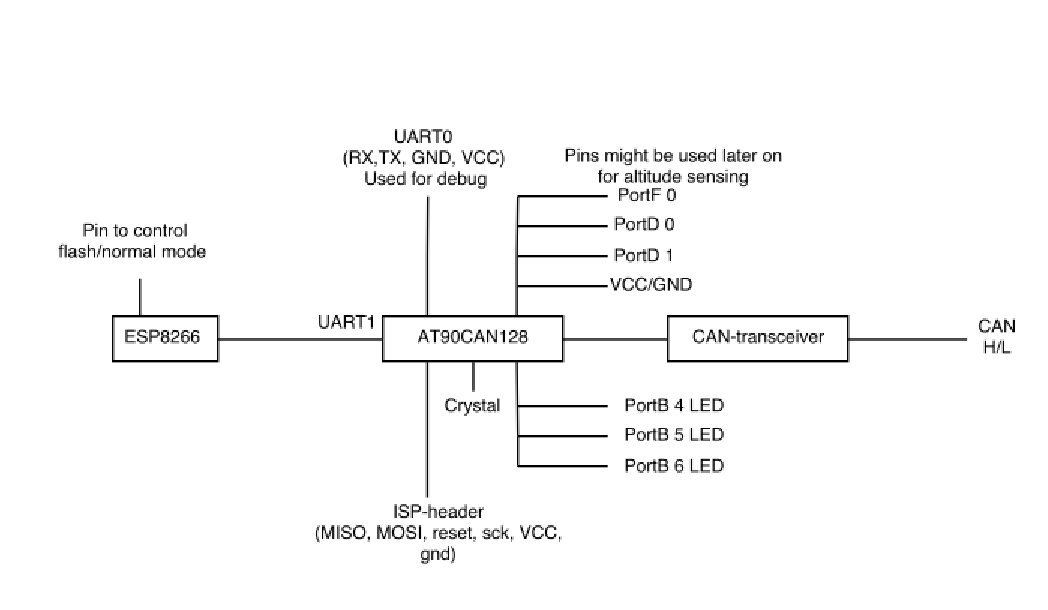
\includegraphics[width=1\textwidth]{graphics/PCB_block_v3.eps}
    \caption{Block schematic of the WIFI-extentionboard developed to AQ M4}
    \label{fig:PCB_block}
\end{figure}

\subsubsection{ATmega}
\subsubsection{Wireless Communication}
An important part of the hardware is the wireless communication used between the PC and the drones.
The wireless communication mpodule has severel requirements it needs to fulfill in order to make the whole system work as expected. A comparesiontable has been made in table \ref{tab:compare_table_wireless_communication} to find the wireless communication module that is best suited for the task.


\begin{table}[H]
	\centering
	\begin{tabular}{@{}|l|l|l|l|l|l|l|@{}}
		\toprule
		\textbf{Product} & \textbf{Size} & \textbf{Price} & 				\textbf{Usability} & \textbf{Power consumption} & 					\textbf{Range} & \textbf{Score} \\ \midrule
		ESP8266          &               &                &                    		&                            &                &                		\\ \midrule
		EMW3165          &               &                &                    		&                            &                &                		\\ \midrule
		nRF51822         &               &                &                    		&                            &                &                		\\ \bottomrule
	\end{tabular}
	\caption{Comparisontable used to compare different wireless 		communication modules}
	\label{tab:compare_table_wireless_communication}
\end{table}

\subsubsection{Pins}
A few pins where made available through solder pads for easy access if needed later on.

The following pins where available as solder pads:
\begin{itemize}
	\item PortF 0 - Alternative function as ADC, channel 0
	\item PortD 0 - Alternative function as interrupt, INT0
	\item PortD 1 - Alternative function as interrupt, INT1
\end{itemize}
In case the onboard baromter isn't accurate enough, an alternative distance could be used to measure the drones altitude with respect to the ground.
PortF0 has been made available since some distance sensors give output as an analogue value. 
An example of such sensor is an Infrared proximity sensor.\footnote{http://www.sharpsma.com/webfm\_send/1208} \\
As an alternative type of distance sensor, a ultrasoinc could be used such as HCSR04.
As output it gives a binary output with high-time proportional with the distance.\footnote{http://www.micropik.com/PDF/HCSR04.pdf}.
To detect the high-time, one of PortD1/0 would be useful. \\

Which type of sensor suits best as a distance sensor to provice altitude information to the drone is ouf of the scope of this report. The PCB has just been made ready to different types of sensors.

\subsubsection{Debug/ISP}
In the final schematic UART0 and ISP pins where combined in one pinheader for easy access through one cable. \Mathias{Refer to image of board}
To program the AtMega the ISP pins where required to be easy accessable. 
UART0 was made accessable to be used as debug and programming of the ESP8266 board.
The plan was to setup the AtMega as UART passthrough from UART0 to UART1.
Due to a mistake\footnote{The wrong pair of MISO/MOSI pins where made available in the ISP-header. The correct pair of MISO/MOSI is also RXD0/TXD0 as alternative function} in the final schematic, both UART0 and UART1 where made accessable trough the ISP/debug header. 
This ended up making it easier to program the ESP8266-board without using the AtMega as UART passthrough.

\newpage